\documentclass[tikz]{standalone}

\usepackage{amsmath,bm,amssymb}
\usepackage{pgfplots}
\usepackage{vector} % package included in this directory

\pgfplotsset{compat=newest}
\pgfplotsset{every axis legend/.append style={%
  cells={anchor=west}}
}

\usetikzlibrary{arrows}
\usetikzlibrary{calc}

\tikzset{>=stealth'}

\usepgfplotslibrary{fillbetween}
\usepgfplotslibrary{groupplots}

\definecolor{pastelMagenta}{HTML}{FF48CF}
\definecolor{pastelPurple}{HTML}{8770FE}
\definecolor{pastelBlue}{HTML}{1BA1EA}
\definecolor{pastelSeaGreen}{HTML}{14B57F}
\definecolor{pastelGreen}{HTML}{3EAA0D}
\definecolor{pastelOrange}{HTML}{C38D09}
\definecolor{pastelRed}{HTML}{F5615C}

\newcommand{\transpose}{\top}
\newcommand{\mat}[1]{\vect{#1}}
\renewcommand{\vec}[1]{\vect{#1}}

% static u8 MAPDATA[8*8] = {
%     1, 1, 1, 1, 1, 1, 1, 1,
%     1, 0, 0, 0, 0, 0, 0, 1,
%     1, 0, 0, 3, 0, 0, 4, 1,
%     1, 0, 0, 0, 0, 0, 0, 1,
%     1, 0, 0, 0, 0, 0, 4, 1,
%     1, 0, 2, 0, 0, 0, 0, 1,
%     1, 0, 0, 0, 0, 0, 0, 1,
%     1, 1, 1, 1, 1, 1, 1, 1,
% }; green yellow red

\begin{document}
  % \begin{tikzpicture}[x=1cm, y=1cm]
  %   \draw[draw=white, fill=pastelBlue] (0,0) rectangle ++ (1,1);
  %   \draw[draw=white, fill=pastelBlue] (1,0) rectangle ++ (1,1);
  %   \draw[draw=white, fill=pastelBlue] (2,0) rectangle ++ (1,1);
  %   \draw[draw=white, fill=pastelBlue] (3,0) rectangle ++ (1,1);
  %   \draw[draw=white, fill=pastelBlue] (4,0) rectangle ++ (1,1);
  %   \draw[draw=white, fill=pastelBlue] (5,0) rectangle ++ (1,1);
  %   \draw[draw=white, fill=pastelBlue] (6,0) rectangle ++ (1,1);
  %   \draw[draw=white, fill=pastelBlue] (7,0) rectangle ++ (1,1);

  %   \draw[draw=white, fill=pastelBlue] (0,1) rectangle ++ (1,1);
  %   \draw[draw=white, fill=black!10]   (1,1) rectangle ++ (1,1);
  %   \draw[draw=white, fill=black!10]   (2,1) rectangle ++ (1,1);
  %   \draw[draw=white, fill=black!10]   (3,1) rectangle ++ (1,1);
  %   \draw[draw=white, fill=black!10]   (4,1) rectangle ++ (1,1);
  %   \draw[draw=white, fill=black!10]   (5,1) rectangle ++ (1,1);
  %   \draw[draw=white, fill=black!10]   (6,1) rectangle ++ (1,1);
  %   \draw[draw=white, fill=pastelBlue] (7,1) rectangle ++ (1,1);

  %   \draw[draw=white, fill=pastelBlue]  (0,2) rectangle ++ (1,1);
  %   \draw[draw=white, fill=black!10]    (1,2) rectangle ++ (1,1);
  %   \draw[draw=white, fill=black!10]    (2,2) rectangle ++ (1,1);
  %   \draw[draw=white, fill=black!10]    (3,2) rectangle ++ (1,1);
  %   \draw[draw=white, fill=black!10]    (4,2) rectangle ++ (1,1);
  %   \draw[draw=white, fill=pastelGreen] (5,2) rectangle ++ (1,1);
  %   \draw[draw=white, fill=black!10]    (6,2) rectangle ++ (1,1);
  %   \draw[draw=white, fill=pastelBlue]  (7,2) rectangle ++ (1,1);

  %   \draw[draw=white, fill=pastelBlue] (0,3) rectangle ++ (1,1);
  %   \draw[draw=white, fill=pastelRed]  (1,3) rectangle ++ (1,1);
  %   \draw[draw=white, fill=black!10]   (2,3) rectangle ++ (1,1);
  %   \draw[draw=white, fill=black!10]   (3,3) rectangle ++ (1,1);
  %   \draw[draw=white, fill=black!10]   (4,3) rectangle ++ (1,1);
  %   \draw[draw=white, fill=black!10]   (5,3) rectangle ++ (1,1);
  %   \draw[draw=white, fill=black!10]   (6,3) rectangle ++ (1,1);
  %   \draw[draw=white, fill=pastelBlue] (7,3) rectangle ++ (1,1);

  %   \draw[draw=white, fill=pastelBlue] (0,4) rectangle ++ (1,1);
  %   \draw[draw=white, fill=black!10]   (1,4) rectangle ++ (1,1);
  %   \draw[draw=white, fill=black!10]   (2,4) rectangle ++ (1,1);
  %   \draw[draw=white, fill=black!10]   (3,4) rectangle ++ (1,1);
  %   \draw[draw=white, fill=black!10]   (4,4) rectangle ++ (1,1);
  %   \draw[draw=white, fill=black!10]   (5,4) rectangle ++ (1,1);
  %   \draw[draw=white, fill=black!10]   (6,4) rectangle ++ (1,1);
  %   \draw[draw=white, fill=pastelBlue] (7,4) rectangle ++ (1,1);

  %   \draw[draw=white, fill=pastelBlue] (0,5) rectangle ++ (1,1);
  %   \draw[draw=white, fill=pastelRed]  (1,5) rectangle ++ (1,1);
  %   \draw[draw=white, fill=black!10]   (2,5) rectangle ++ (1,1);
  %   \draw[draw=white, fill=black!10]   (3,5) rectangle ++ (1,1);
  %   \draw[draw=white, fill=yellow]     (4,5) rectangle ++ (1,1);
  %   \draw[draw=white, fill=black!10]   (5,5) rectangle ++ (1,1);
  %   \draw[draw=white, fill=black!10]   (6,5) rectangle ++ (1,1);
  %   \draw[draw=white, fill=pastelBlue] (7,5) rectangle ++ (1,1);

  %   \draw[draw=white, fill=pastelBlue] (0,6) rectangle ++ (1,1);
  %   \draw[draw=white, fill=black!10]   (1,6) rectangle ++ (1,1);
  %   \draw[draw=white, fill=black!10]   (2,6) rectangle ++ (1,1);
  %   \draw[draw=white, fill=black!10]   (3,6) rectangle ++ (1,1);
  %   \draw[draw=white, fill=black!10]   (4,6) rectangle ++ (1,1);
  %   \draw[draw=white, fill=black!10]   (5,6) rectangle ++ (1,1);
  %   \draw[draw=white, fill=black!10]   (6,6) rectangle ++ (1,1);
  %   \draw[draw=white, fill=pastelBlue] (7,6) rectangle ++ (1,1);

  %   \draw[draw=white, fill=pastelBlue] (0,7) rectangle ++ (1,1);
  %   \draw[draw=white, fill=pastelBlue] (1,7) rectangle ++ (1,1);
  %   \draw[draw=white, fill=pastelBlue] (2,7) rectangle ++ (1,1);
  %   \draw[draw=white, fill=pastelBlue] (3,7) rectangle ++ (1,1);
  %   \draw[draw=white, fill=pastelBlue] (4,7) rectangle ++ (1,1);
  %   \draw[draw=white, fill=pastelBlue] (5,7) rectangle ++ (1,1);
  %   \draw[draw=white, fill=pastelBlue] (6,7) rectangle ++ (1,1);
  %   \draw[draw=white, fill=pastelBlue] (7,7) rectangle ++ (1,1);

  %   \coordinate (camera) at (5.75, 5.5);
  %   \fill[black] (camera) circle (0.1);
  %   \draw[fill=white] (camera) -- ++(240:0.5) -- ($(camera) + (190:0.5)$) -- cycle;
  %   \draw[->, =stealth'] (camera) -- ++(215:0.7);

  %   \fill[white, opacity=0.5] (camera) -- ++(240:9.5) -- ($(camera) + (190:9.5)$) -- cycle;
  % \end{tikzpicture}

  % \begin{tikzpicture}[x=1cm, y=1cm]
  %   \fill[pastelBlue] (0,0) rectangle ++ (2.5,3);
  %   \fill[black!40] (0,0) rectangle ++(12,-0.1);
  %   \draw (0,0) -- (12,0);
  %   \fill[black!40] (0,3) rectangle ++(12,0.1);
  %   \draw (0,3) -- (12,3);

  %   \draw[line width=0.25cm, black!60, line cap=round] (11,1.25) -- (11,0.75);
  %   \draw[line width=0.25cm, black!60, line cap=round] (11,0.75) -- (10.75,0.1);
  %   \draw[line width=0.25cm, black!60, line cap=round] (11,0.75) -- (11.25,0.1);
  %   \draw[line width=0.25cm, black!60, line cap=round] (11,1.25) -- (10.75,0.75);
  %   \draw[line width=0.25cm, black!60, line cap=round] (11,1.25) -- (11.25,0.75);

  %   \coordinate (camera) at (11, 1.6);
  %   \fill[black!60] (camera) circle (0.35);
  %   \fill[white] (camera) -- ++(160:0.5) -- ($(camera) + (200:0.5)$) -- cycle;
  %   \draw[pastelPurple] (camera) -- ++(160:9.5);
  %   \draw[pastelPurple] (camera) -- ++(200:9.5);

  %   \draw[gray, ultra thick] ($(camera) + (160:1.0)$) -- ($(camera) + (200:1.0)$);
  %   \node[anchor=north] at ($(camera) + (200:1.0) + (0,-0.1)$) {screen};

  %   \draw[black, ->, =stealth'] (camera) -- (2.5,2.5);

  %   \draw[pastelBlue, ->, =stealth'] (8,1.45) -> (10,1.7);
  %   \node[anchor=north] at ($(camera) + (-3,-0.1)$) {make this pixel blue};
  % \end{tikzpicture}

  % \begin{tikzpicture}[x=1cm, y=1cm]
  %   \coordinate (camera) at (11, 1.6);
  %   \fill[black!20] (camera) -- (2.5,3.0) -- ($(camera) + (160:4.1)$) -- cycle;
  %   \node at (6,2.75) {\textcolor{white}{ceiling color}};
  %   \fill[pastelBlue!50] (camera) -- (2.5,3.0) -- (2.5,0.0) -- cycle;
  %   \node at (6,1.5) {\textcolor{white}{block color}};
  %   \fill[black!30] (camera) -- (2.5,0.0) -- ($(camera) + (200:4.7)$) -- cycle;
  %   \node at (6,0.3) {\textcolor{white}{floor color}};

  %   \fill[pastelBlue] (0,0) rectangle ++ (2.5,3);
  %   \fill[black!40] (0,0) rectangle ++(12,-0.1);
  %   \draw (0,0) -- (12,0);
  %   \fill[black!40] (0,3) rectangle ++(12,0.1);
  %   \draw (0,3) -- (12,3);

  %   \draw[line width=0.25cm, black!60, line cap=round] (11,1.25) -- (11,0.75);
  %   \draw[line width=0.25cm, black!60, line cap=round] (11,0.75) -- (10.75,0.1);
  %   \draw[line width=0.25cm, black!60, line cap=round] (11,0.75) -- (11.25,0.1);
  %   \draw[line width=0.25cm, black!60, line cap=round] (11,1.25) -- (10.75,0.75);
  %   \draw[line width=0.25cm, black!60, line cap=round] (11,1.25) -- (11.25,0.75);

  %   \fill[black!60] (camera) circle (0.35);
  %   % \fill[white] (camera) -- ++(160:0.5) -- ($(camera) + (200:0.5)$) -- cycle;
  %   \draw[pastelPurple] (camera) -- ++(160:9.5);
  %   \draw[pastelPurple] (camera) -- ++(200:9.5);

  %   \draw[gray, ultra thick] ($(camera) + (160:1.0)$) -- ($(camera) + (200:1.0)$);
  %   \node[anchor=north] at ($(camera) + (200:1.0) + (0,-0.1)$) {screen};


  %   \draw[black] (camera) -- (2.5,0.0);
  %   \draw[black] (camera) -- (2.5,3.0);
  % \end{tikzpicture}

  % \begin{tikzpicture}[x=1cm, y=1cm]
  %   \coordinate (camera) at (11, 1.6);

  %   \fill[pastelBlue] (0,0) rectangle ++ (2.5,3);
  %   \fill[black!40] (0,0) rectangle ++(12,-0.1);
  %   \draw (0,0) -- (12,0);
  %   \fill[black!40] (0,3) rectangle ++(12,0.1);
  %   \draw (0,3) -- (12,3);

  %   \draw[line width=0.25cm, black!60, line cap=round] (11,1.25) -- (11,0.75);
  %   \draw[line width=0.25cm, black!60, line cap=round] (11,0.75) -- (10.75,0.1);
  %   \draw[line width=0.25cm, black!60, line cap=round] (11,0.75) -- (11.25,0.1);
  %   \draw[line width=0.25cm, black!60, line cap=round] (11,1.25) -- (10.75,0.75);
  %   \draw[line width=0.25cm, black!60, line cap=round] (11,1.25) -- (11.25,0.75);

  %   \fill[black!60] (camera) circle (0.35);
  %   % \fill[white] (camera) -- ++(160:0.5) -- ($(camera) + (200:0.5)$) -- cycle;
  %   \draw[pastelPurple] (camera) -- ++(160:9.5);
  %   \draw[pastelPurple] (camera) -- ++(200:9.5);

  %   \draw[gray, ultra thick] ($(camera) + (160:1.0)$) -- ($(camera) + (200:1.0)$);

  %   \draw[black] (camera) -- (2.5,0.0) -- (2.5,3.0) -- cycle;
  %   \draw[black] (camera) -- (2.5,1.6);
  %   \draw[black] (2.65,1.6) -- ++(0,0.15) -- ++(-0.15,0);

  %   \node[anchor=east]  at (2.5,2.25) {$H - z$};
  %   \node[anchor=east]  at (2.5,0.75) {$z$};
  %   \node[anchor=south] at (6.0,1.6) {$\ell$};

  %   \node[anchor=east]  at (8.5,1.3) {$z'$};
  %   \node[anchor=east]  at (8.5,1.8) {$z''$};
  %   \draw[->, =stealth'] (8.5,1.3) -- ($(camera) + (185:1.0)$);
  %   \draw[->, =stealth'] (8.5,1.8) -- ($(camera) + (175:1.0)$);
  % \end{tikzpicture}

  % \begin{tikzpicture}[x=1cm, y=1cm]
  %   \draw[draw=white, fill=pastelBlue] (0,0) rectangle ++ (1,1);
  %   \draw[draw=white, fill=pastelBlue] (1,0) rectangle ++ (1,1);
  %   \draw[draw=white, fill=pastelBlue] (2,0) rectangle ++ (1,1);
  %   \draw[draw=white, fill=pastelBlue] (3,0) rectangle ++ (1,1);
  %   \draw[draw=white, fill=pastelBlue] (4,0) rectangle ++ (1,1);
  %   \draw[draw=white, fill=pastelBlue] (5,0) rectangle ++ (1,1);
  %   \draw[draw=white, fill=pastelBlue] (6,0) rectangle ++ (1,1);
  %   \draw[draw=white, fill=pastelBlue] (7,0) rectangle ++ (1,1);

  %   \draw[draw=white, fill=pastelBlue] (0,1) rectangle ++ (1,1);
  %   \draw[draw=white, fill=black!10]   (1,1) rectangle ++ (1,1);
  %   \draw[draw=white, fill=black!10]   (2,1) rectangle ++ (1,1);
  %   \draw[draw=white, fill=black!10]   (3,1) rectangle ++ (1,1);
  %   \draw[draw=white, fill=black!10]   (4,1) rectangle ++ (1,1);
  %   \draw[draw=white, fill=black!10]   (5,1) rectangle ++ (1,1);
  %   \draw[draw=white, fill=black!10]   (6,1) rectangle ++ (1,1);
  %   \draw[draw=white, fill=pastelBlue] (7,1) rectangle ++ (1,1);

  %   \draw[draw=white, fill=pastelBlue]  (0,2) rectangle ++ (1,1);
  %   \draw[draw=white, fill=black!10]    (1,2) rectangle ++ (1,1);
  %   \draw[draw=white, fill=black!10]    (2,2) rectangle ++ (1,1);
  %   \draw[draw=white, fill=black!10]    (3,2) rectangle ++ (1,1);
  %   \draw[draw=white, fill=black!10]    (4,2) rectangle ++ (1,1);
  %   \draw[draw=white, fill=pastelGreen] (5,2) rectangle ++ (1,1);
  %   \draw[draw=white, fill=black!10]    (6,2) rectangle ++ (1,1);
  %   \draw[draw=white, fill=pastelBlue]  (7,2) rectangle ++ (1,1);

  %   \draw[draw=white, fill=pastelBlue] (0,3) rectangle ++ (1,1);
  %   \draw[draw=white, fill=pastelRed]  (1,3) rectangle ++ (1,1);
  %   \draw[draw=white, fill=black!10]   (2,3) rectangle ++ (1,1);
  %   \draw[draw=white, fill=black!10]   (3,3) rectangle ++ (1,1);
  %   \draw[draw=white, fill=black!10]   (4,3) rectangle ++ (1,1);
  %   \draw[draw=white, fill=black!10]   (5,3) rectangle ++ (1,1);
  %   \draw[draw=white, fill=black!10]   (6,3) rectangle ++ (1,1);
  %   \draw[draw=white, fill=pastelBlue] (7,3) rectangle ++ (1,1);

  %   \draw[draw=white, fill=pastelBlue] (0,4) rectangle ++ (1,1);
  %   \draw[draw=white, fill=black!10]   (1,4) rectangle ++ (1,1);
  %   \draw[draw=white, fill=black!10]   (2,4) rectangle ++ (1,1);
  %   \draw[draw=white, fill=black!10]   (3,4) rectangle ++ (1,1);
  %   \draw[draw=white, fill=black!10]   (4,4) rectangle ++ (1,1);
  %   \draw[draw=white, fill=black!10]   (5,4) rectangle ++ (1,1);
  %   \draw[draw=white, fill=black!10]   (6,4) rectangle ++ (1,1);
  %   \draw[draw=white, fill=pastelBlue] (7,4) rectangle ++ (1,1);

  %   \draw[draw=white, fill=pastelBlue] (0,5) rectangle ++ (1,1);
  %   \draw[draw=white, fill=pastelRed]  (1,5) rectangle ++ (1,1);
  %   \draw[draw=white, fill=black!10]   (2,5) rectangle ++ (1,1);
  %   \draw[draw=white, fill=black!10]   (3,5) rectangle ++ (1,1);
  %   \draw[draw=white, fill=yellow]     (4,5) rectangle ++ (1,1);
  %   \draw[draw=white, fill=black!10]   (5,5) rectangle ++ (1,1);
  %   \draw[draw=white, fill=black!10]   (6,5) rectangle ++ (1,1);
  %   \draw[draw=white, fill=pastelBlue] (7,5) rectangle ++ (1,1);

  %   \draw[draw=white, fill=pastelBlue] (0,6) rectangle ++ (1,1);
  %   \draw[draw=white, fill=black!10]   (1,6) rectangle ++ (1,1);
  %   \draw[draw=white, fill=black!10]   (2,6) rectangle ++ (1,1);
  %   \draw[draw=white, fill=black!10]   (3,6) rectangle ++ (1,1);
  %   \draw[draw=white, fill=black!10]   (4,6) rectangle ++ (1,1);
  %   \draw[draw=white, fill=black!10]   (5,6) rectangle ++ (1,1);
  %   \draw[draw=white, fill=black!10]   (6,6) rectangle ++ (1,1);
  %   \draw[draw=white, fill=pastelBlue] (7,6) rectangle ++ (1,1);

  %   \draw[draw=white, fill=pastelBlue] (0,7) rectangle ++ (1,1);
  %   \draw[draw=white, fill=pastelBlue] (1,7) rectangle ++ (1,1);
  %   \draw[draw=white, fill=pastelBlue] (2,7) rectangle ++ (1,1);
  %   \draw[draw=white, fill=pastelBlue] (3,7) rectangle ++ (1,1);
  %   \draw[draw=white, fill=pastelBlue] (4,7) rectangle ++ (1,1);
  %   \draw[draw=white, fill=pastelBlue] (5,7) rectangle ++ (1,1);
  %   \draw[draw=white, fill=pastelBlue] (6,7) rectangle ++ (1,1);
  %   \draw[draw=white, fill=pastelBlue] (7,7) rectangle ++ (1,1);

  %   \coordinate (camera) at (5.75, 5.5);
  %   \fill[black] (camera) circle (0.1);
  %   \draw[fill=white] (camera) -- ++(240:0.5) -- ($(camera) + (190:0.5)$) -- cycle;
  %   \draw[->, =stealth'] (camera) -- ++(215:0.7);

  %   \fill[white, opacity=0.5] (camera) -- ++(240:9.5) -- ($(camera) + (190:9.5)$) -- cycle;

  %   \draw[black, ->, =stealth'] (camera) -- (2.25, 1);
  %   \node at (3.8,3.3) {$\ell$};
  % \end{tikzpicture}

  % \begin{tikzpicture}[x=1cm, y=1cm]
  %   \draw[draw=white, fill=pastelBlue] (0,0) rectangle ++ (1,1);
  %   \draw[draw=white, fill=pastelBlue] (1,0) rectangle ++ (1,1);
  %   \draw[draw=white, fill=pastelBlue] (2,0) rectangle ++ (1,1);
  %   \draw[draw=white, fill=pastelBlue] (3,0) rectangle ++ (1,1);
  %   \draw[draw=white, fill=pastelBlue] (4,0) rectangle ++ (1,1);
  %   \draw[draw=white, fill=pastelBlue] (5,0) rectangle ++ (1,1);
  %   \draw[draw=white, fill=pastelBlue] (6,0) rectangle ++ (1,1);
  %   \draw[draw=white, fill=pastelBlue] (7,0) rectangle ++ (1,1);

  %   \draw[draw=white, fill=pastelBlue] (0,1) rectangle ++ (1,1);
  %   \draw[draw=white, fill=black!10]   (1,1) rectangle ++ (1,1);
  %   \draw[draw=white, fill=black!10]   (2,1) rectangle ++ (1,1);
  %   \draw[draw=white, fill=black!10]   (3,1) rectangle ++ (1,1);
  %   \draw[draw=white, fill=black!10]   (4,1) rectangle ++ (1,1);
  %   \draw[draw=white, fill=black!10]   (5,1) rectangle ++ (1,1);
  %   \draw[draw=white, fill=black!10]   (6,1) rectangle ++ (1,1);
  %   \draw[draw=white, fill=pastelBlue] (7,1) rectangle ++ (1,1);

  %   \draw[draw=white, fill=pastelBlue]  (0,2) rectangle ++ (1,1);
  %   \draw[draw=white, fill=black!10]    (1,2) rectangle ++ (1,1);
  %   \draw[draw=white, fill=black!10]    (2,2) rectangle ++ (1,1);
  %   \draw[draw=white, fill=black!10]    (3,2) rectangle ++ (1,1);
  %   \draw[draw=white, fill=black!10]    (4,2) rectangle ++ (1,1);
  %   \draw[draw=white, fill=pastelGreen] (5,2) rectangle ++ (1,1);
  %   \draw[draw=white, fill=black!10]    (6,2) rectangle ++ (1,1);
  %   \draw[draw=white, fill=pastelBlue]  (7,2) rectangle ++ (1,1);

  %   \draw[draw=white, fill=pastelBlue] (0,3) rectangle ++ (1,1);
  %   \draw[draw=white, fill=pastelRed]  (1,3) rectangle ++ (1,1);
  %   \draw[draw=white, fill=black!10]   (2,3) rectangle ++ (1,1);
  %   \draw[draw=white, fill=black!10]   (3,3) rectangle ++ (1,1);
  %   \draw[draw=white, fill=black!10]   (4,3) rectangle ++ (1,1);
  %   \draw[draw=white, fill=black!10]   (5,3) rectangle ++ (1,1);
  %   \draw[draw=white, fill=black!10]   (6,3) rectangle ++ (1,1);
  %   \draw[draw=white, fill=pastelBlue] (7,3) rectangle ++ (1,1);

  %   \draw[draw=white, fill=pastelBlue] (0,4) rectangle ++ (1,1);
  %   \draw[draw=white, fill=black!10]   (1,4) rectangle ++ (1,1);
  %   \draw[draw=white, fill=black!10]   (2,4) rectangle ++ (1,1);
  %   \draw[draw=white, fill=black!10]   (3,4) rectangle ++ (1,1);
  %   \draw[draw=white, fill=black!10]   (4,4) rectangle ++ (1,1);
  %   \draw[draw=white, fill=black!10]   (5,4) rectangle ++ (1,1);
  %   \draw[draw=white, fill=black!10]   (6,4) rectangle ++ (1,1);
  %   \draw[draw=white, fill=pastelBlue] (7,4) rectangle ++ (1,1);

  %   \draw[draw=white, fill=pastelBlue] (0,5) rectangle ++ (1,1);
  %   \draw[draw=white, fill=pastelRed]  (1,5) rectangle ++ (1,1);
  %   \draw[draw=white, fill=black!10]   (2,5) rectangle ++ (1,1);
  %   \draw[draw=white, fill=black!10]   (3,5) rectangle ++ (1,1);
  %   \draw[draw=white, fill=yellow]     (4,5) rectangle ++ (1,1);
  %   \draw[draw=white, fill=black!10]   (5,5) rectangle ++ (1,1);
  %   \draw[draw=white, fill=black!10]   (6,5) rectangle ++ (1,1);
  %   \draw[draw=white, fill=pastelBlue] (7,5) rectangle ++ (1,1);

  %   \draw[draw=white, fill=pastelBlue] (0,6) rectangle ++ (1,1);
  %   \draw[draw=white, fill=black!10]   (1,6) rectangle ++ (1,1);
  %   \draw[draw=white, fill=black!10]   (2,6) rectangle ++ (1,1);
  %   \draw[draw=white, fill=black!10]   (3,6) rectangle ++ (1,1);
  %   \draw[draw=white, fill=black!10]   (4,6) rectangle ++ (1,1);
  %   \draw[draw=white, fill=black!10]   (5,6) rectangle ++ (1,1);
  %   \draw[draw=white, fill=black!10]   (6,6) rectangle ++ (1,1);
  %   \draw[draw=white, fill=pastelBlue] (7,6) rectangle ++ (1,1);

  %   \draw[draw=white, fill=pastelBlue] (0,7) rectangle ++ (1,1);
  %   \draw[draw=white, fill=pastelBlue] (1,7) rectangle ++ (1,1);
  %   \draw[draw=white, fill=pastelBlue] (2,7) rectangle ++ (1,1);
  %   \draw[draw=white, fill=pastelBlue] (3,7) rectangle ++ (1,1);
  %   \draw[draw=white, fill=pastelBlue] (4,7) rectangle ++ (1,1);
  %   \draw[draw=white, fill=pastelBlue] (5,7) rectangle ++ (1,1);
  %   \draw[draw=white, fill=pastelBlue] (6,7) rectangle ++ (1,1);
  %   \draw[draw=white, fill=pastelBlue] (7,7) rectangle ++ (1,1);

  %   \coordinate (camera) at (5.75, 5.5);
  %   \coordinate (base) at (5, 5);
  %   \fill[black] (camera) circle (0.1);
  %   \fill[gray] (base) circle (0.07);
  %   \draw[gray, ->] (base) -- ++(0.75,0) node [black,midway,yshift=-2.5] {\scriptsize $x_\text{rem}$};
  %   \draw[gray, ->] ($(base) + (0.75,0)$) -- ++(0,0.5) node [black,midway,xshift=8.5] {\scriptsize $y_\text{rem}$};
  %   \node[anchor=north east] at (base) {\scriptsize $(x_\text{ind}, y_\text{ind})$};
  %   % \draw[fill=white] (camera) -- ++(240:0.5) -- ($(camera) + (190:0.5)$) -- cycle;
  %   % \draw[->, =stealth'] (camera) -- ++(215:0.7);

  %   % \fill[white, opacity=0.5] (camera) -- ++(240:9.5) -- ($(camera) + (190:9.5)$) -- cycle;

  %   % \draw[black, ->, =stealth'] (camera) -- (2.25, 1);
  %   % \node at (3.8,3.3) {$\ell$};
  % \end{tikzpicture}

  % \begin{tikzpicture}[x=1cm, y=1cm]
  %   \coordinate (camera) at (1, 1);
  %   \coordinate (pixel) at ($(camera) + (240:0.64)$);
  %   \fill[black] (camera) circle (0.03);
  %   \draw[black, ->] (camera) -- ++(225:0.25);
  %   \draw[black] (camera) -- ++(260:0.75) -- ($(camera) + (190:0.75)$) -- cycle;
  %   \draw[gray, thick] ($(camera) + (260:0.75)$) -- ($(camera) + (190:0.75)$);
  %   \fill[pastelBlue] (pixel) circle (0.03);
  %   \draw[pastelBlue, ->] (camera) -- ++(240:2.0);

  %   \draw[pastelPurple] ($(camera) + (315:0.75)$) -- ++(225:0.6);
  %   \draw[pastelPurple] ($(camera) + (315:0.7)$) -- ($(camera) + (315:0.8)$);
  %   \draw[pastelPurple] ($(camera) + (315:0.7) + (225:0.6)$) -- ($(camera) + (315:0.8) + (225:0.6)$);
  %   \node[anchor=north west, xshift=-1.5, yshift=1.5] at ($(camera) + (315:0.7) + (225:0.3)$) {\tiny $d$};

  %   \draw[pastelPurple] ($(camera) + (260:0.75) + (225:0.2)$) -- ($(camera) + (190:0.75) + (225:0.2)$) node [black, midway, xshift=-2, yshift=-2] {\tiny $w$};
  %   \draw[pastelPurple] ($(camera) + (190:0.75) + (225:0.15)$) -- ($(camera) + (190:0.75) + (225:0.25)$);
  %   \draw[pastelPurple] ($(camera) + (260:0.75) + (225:0.15)$) -- ($(camera) + (260:0.75) + (225:0.25)$);

  %   \draw[pastelPurple] ($(pixel) + (225:0.4)$) -- ($(camera) + (260:0.75) + (225:0.4)$) node [black, midway, xshift=1.5, yshift=-5] {\tiny $w'$};
  %   \draw[pastelPurple] ($(camera) + (260:0.75) + (225:0.35)$) -- ($(camera) + (260:0.75) + (225:0.45)$);
  %   \draw[pastelPurple] ($(pixel) + (225:0.35)$) -- ($(pixel) + (225:0.45)$);

  %   \node[anchor=west, xshift=-2] at (camera) {\tiny $\boldsymbol{c}$};
  %   \node[anchor=west, xshift=-2] at (pixel) {\tiny $\boldsymbol{p}$};
  %   \node[anchor=east, xshift=2] at ($(camera) + (225:0.25)$) {\tiny $\hat{\boldsymbol{b}}$};
  % \end{tikzpicture}

  % \begin{tikzpicture}[x=1cm, y=1cm]
  %   \draw[draw=white, fill=pastelBlue] (0,0) rectangle ++ (1,1);
  %   \draw[draw=white, fill=pastelBlue] (1,0) rectangle ++ (1,1);
  %   \draw[draw=white, fill=pastelBlue] (2,0) rectangle ++ (1,1);
  %   \draw[draw=white, fill=pastelBlue] (3,0) rectangle ++ (1,1);
  %   \draw[draw=white, fill=pastelBlue] (4,0) rectangle ++ (1,1);
  %   \draw[draw=white, fill=pastelBlue] (5,0) rectangle ++ (1,1);
  %   \draw[draw=white, fill=pastelBlue] (6,0) rectangle ++ (1,1);
  %   \draw[draw=white, fill=pastelBlue] (7,0) rectangle ++ (1,1);

  %   \draw[draw=white, fill=pastelBlue] (0,1) rectangle ++ (1,1);
  %   \draw[draw=white, fill=black!10]   (1,1) rectangle ++ (1,1);
  %   \draw[draw=white, fill=black!10]   (2,1) rectangle ++ (1,1);
  %   \draw[draw=white, fill=black!10]   (3,1) rectangle ++ (1,1);
  %   \draw[draw=white, fill=black!10]   (4,1) rectangle ++ (1,1);
  %   \draw[draw=white, fill=black!10]   (5,1) rectangle ++ (1,1);
  %   \draw[draw=white, fill=black!10]   (6,1) rectangle ++ (1,1);
  %   \draw[draw=white, fill=pastelBlue] (7,1) rectangle ++ (1,1);

  %   \draw[draw=white, fill=pastelBlue]  (0,2) rectangle ++ (1,1);
  %   \draw[draw=white, fill=black!10]    (1,2) rectangle ++ (1,1);
  %   \draw[draw=white, fill=black!10]    (2,2) rectangle ++ (1,1);
  %   \draw[draw=white, fill=black!10]    (3,2) rectangle ++ (1,1);
  %   \draw[draw=white, fill=black!10]    (4,2) rectangle ++ (1,1);
  %   \draw[draw=white, fill=pastelGreen] (5,2) rectangle ++ (1,1);
  %   \draw[draw=white, fill=black!10]    (6,2) rectangle ++ (1,1);
  %   \draw[draw=white, fill=pastelBlue]  (7,2) rectangle ++ (1,1);

  %   \draw[draw=white, fill=pastelBlue] (0,3) rectangle ++ (1,1);
  %   \draw[draw=white, fill=pastelRed]  (1,3) rectangle ++ (1,1);
  %   \draw[draw=white, fill=black!10]   (2,3) rectangle ++ (1,1);
  %   \draw[draw=white, fill=black!10]   (3,3) rectangle ++ (1,1);
  %   \draw[draw=white, fill=black!10]   (4,3) rectangle ++ (1,1);
  %   \draw[draw=white, fill=black!10]   (5,3) rectangle ++ (1,1);
  %   \draw[draw=white, fill=black!10]   (6,3) rectangle ++ (1,1);
  %   \draw[draw=white, fill=pastelBlue] (7,3) rectangle ++ (1,1);

  %   \draw[draw=white, fill=pastelBlue] (0,4) rectangle ++ (1,1);
  %   \draw[draw=white, fill=black!10]   (1,4) rectangle ++ (1,1);
  %   \draw[draw=white, fill=black!10]   (2,4) rectangle ++ (1,1);
  %   \draw[draw=white, fill=black!10]   (3,4) rectangle ++ (1,1);
  %   \draw[draw=white, fill=black!10]   (4,4) rectangle ++ (1,1);
  %   \draw[draw=white, fill=black!10]   (5,4) rectangle ++ (1,1);
  %   \draw[draw=white, fill=black!10]   (6,4) rectangle ++ (1,1);
  %   \draw[draw=white, fill=pastelBlue] (7,4) rectangle ++ (1,1);

  %   \draw[draw=white, fill=pastelBlue] (0,5) rectangle ++ (1,1);
  %   \draw[draw=white, fill=pastelRed]  (1,5) rectangle ++ (1,1);
  %   \draw[draw=white, fill=black!10]   (2,5) rectangle ++ (1,1);
  %   \draw[draw=white, fill=black!10]   (3,5) rectangle ++ (1,1);
  %   \draw[draw=white, fill=yellow]     (4,5) rectangle ++ (1,1);
  %   \draw[draw=white, fill=black!10]   (5,5) rectangle ++ (1,1);
  %   \draw[draw=white, fill=black!10]   (6,5) rectangle ++ (1,1);
  %   \draw[draw=white, fill=pastelBlue] (7,5) rectangle ++ (1,1);

  %   \draw[draw=white, fill=pastelBlue] (0,6) rectangle ++ (1,1);
  %   \draw[draw=white, fill=black!10]   (1,6) rectangle ++ (1,1);
  %   \draw[draw=white, fill=black!10]   (2,6) rectangle ++ (1,1);
  %   \draw[draw=white, fill=black!10]   (3,6) rectangle ++ (1,1);
  %   \draw[draw=white, fill=black!10]   (4,6) rectangle ++ (1,1);
  %   \draw[draw=white, fill=black!10]   (5,6) rectangle ++ (1,1);
  %   \draw[draw=white, fill=black!10]   (6,6) rectangle ++ (1,1);
  %   \draw[draw=white, fill=pastelBlue] (7,6) rectangle ++ (1,1);

  %   \draw[draw=white, fill=pastelBlue] (0,7) rectangle ++ (1,1);
  %   \draw[draw=white, fill=pastelBlue] (1,7) rectangle ++ (1,1);
  %   \draw[draw=white, fill=pastelBlue] (2,7) rectangle ++ (1,1);
  %   \draw[draw=white, fill=pastelBlue] (3,7) rectangle ++ (1,1);
  %   \draw[draw=white, fill=pastelBlue] (4,7) rectangle ++ (1,1);
  %   \draw[draw=white, fill=pastelBlue] (5,7) rectangle ++ (1,1);
  %   \draw[draw=white, fill=pastelBlue] (6,7) rectangle ++ (1,1);
  %   \draw[draw=white, fill=pastelBlue] (7,7) rectangle ++ (1,1);

  %   \coordinate (camera) at (5.75, 5.5);
  %   \fill[black] (camera) circle (0.1);
  %   \draw[->, =stealth'] (camera) -- ++(240:5.1);

  %   \draw[black, fill=white] (5.461, 5.000) circle (0.06);
  %   \draw[black, fill=white] (5.000, 4.201) circle (0.06);
  %   \draw[black, fill=white] (4.884, 4.000) circle (0.06);
  %   \draw[black, fill=white] (4.307, 3.000) circle (0.06);
  %   \draw[black, fill=white] (4.000, 2.469) circle (0.06);
  %   \draw[black, fill=white] (3.729, 2.000) circle (0.06);
  %   \draw[black, fill=white] (3.152, 1.000) circle (0.06);

  %   \coordinate (intersect) at (3.152, 1.000);
  %   \node at ($(intersect) + (0,-0.3)$) {\scriptsize $x_\text{rem}$};
  %   \draw[magenta, thick] ($(3,1) + (0,-0.15)$) -- ($(intersect) + (0,-0.15)$);
  %   \draw[magenta, thick] ($(3,1) + (0,-0.15) + (0,-0.05)$) -- ($(3,1) + (0,-0.15) + (0,+0.05)$);
  %   \draw[magenta, thick] ($(intersect) + (0,-0.15) + (0,-0.05)$) -- ($(intersect) + (0,-0.15) + (0,+0.05)$);

  %   % dir = [cosd(240), sind(240)] = [-0.5, -0.866]
  %   % dx_a = 2.0
  %   % dx_b = 0
  %   % dy_a = 1.1547
  %   % dy_b = 0

  %   % dt_x = dx_a*x_rem + dx_b
  %   % dt_y = dy_a*y_rem + dy_b

  %   % TILE_WIDTH = 1.0
  %   % x_ind = 5
  %   % y_ind = 5
  %   % n_steps = 0
  %   % while (n_steps < 10)
  %   %   n_steps += 1;

  %   %   dt_best = 99999.0;
  %   %   dx_ind = 0
  %   %   dy_ind = 0

  %   %   dt_x = dx_a*x_rem + dx_b
  %   %   dt_y = dy_a*y_rem + dy_b
  %   %   if dt_x < dt_y
  %   %       dt_best = dt_x
  %   %       dx_ind = dx_ind_dir
  %   %       dy_ind = 0
  %   %   else
  %   %       dt_best = dt_y
  %   %       dx_ind = 0
  %   %       dy_ind = dy_ind_dir
  %   %   end

  %   %   x_ind += dx_ind
  %   %   y_ind += dy_ind
  %   %   x_rem += dir[1] * dt_best - TILE_WIDTH*dx_ind
  %   %   y_rem += dir[2] * dt_best - TILE_WIDTH*dy_ind

  %   %   println(x_ind, ", ", y_ind, ", ", x_rem, ", ", y_rem)
  %   % end

  %   % \fill[white, opacity=0.5] (camera) -- ++(240:9.5) -- ($(camera) + (190:9.5)$) -- cycle;

  %   % \draw[black, ->, =stealth'] (camera) -- (2.25, 1);
  %   % \node at (3.8,3.3) {$\ell$};
  % \end{tikzpicture}

  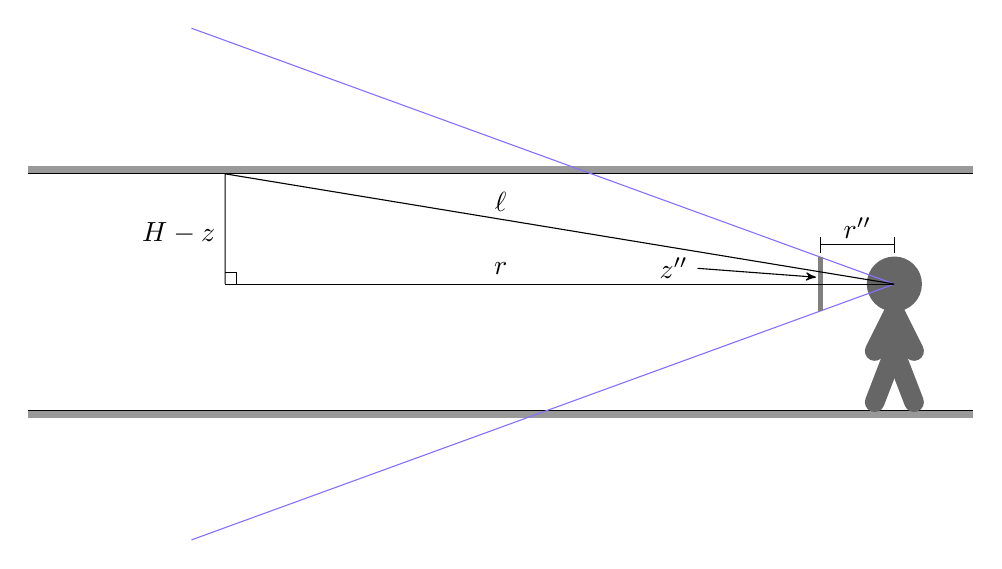
\begin{tikzpicture}[x=1cm, y=1cm]
    \coordinate (camera) at (11, 1.6);

    \fill[black!40] (0,0) rectangle ++(12,-0.1);
    \draw (0,0) -- (12,0);
    \fill[black!40] (0,3) rectangle ++(12,0.1);
    \draw (0,3) -- (12,3);

    \draw[line width=0.25cm, black!60, line cap=round] (11,1.25) -- (11,0.75);
    \draw[line width=0.25cm, black!60, line cap=round] (11,0.75) -- (10.75,0.1);
    \draw[line width=0.25cm, black!60, line cap=round] (11,0.75) -- (11.25,0.1);
    \draw[line width=0.25cm, black!60, line cap=round] (11,1.25) -- (10.75,0.75);
    \draw[line width=0.25cm, black!60, line cap=round] (11,1.25) -- (11.25,0.75);

    \fill[black!60] (camera) circle (0.35);
    % \fill[white] (camera) -- ++(160:0.5) -- ($(camera) + (200:0.5)$) -- cycle;
    \draw[pastelPurple] (camera) -- ++(160:9.5);
    \draw[pastelPurple] (camera) -- ++(200:9.5);

    \draw[gray, ultra thick] ($(camera) + (160:1.0)$) -- ($(camera) + (200:1.0)$);

    \draw[black] (camera) -- (2.5,3.0) -- (2.5, 1.6);
    \draw[black] (camera) -- (2.5,1.6);
    \draw[black] (2.65,1.6) -- ++(0,0.15) -- ++(-0.15,0);

    \draw[black] ($(camera) + (0,0.5)$) -- ($(camera) + (-0.9396, 0) + (0,0.5)$) node [black,midway,yshift=6] {$r''$};
    \draw[black] ($(camera) + (0,0.4)$) -- ($(camera) + (0,0.6)$);
    \draw[black] ($(camera) + (-0.9396,0.4)$) -- ($(camera) + (-0.9396,0.6)$);

    \node[anchor=east]  at (2.5,2.25) {$H - z$};
    \node[anchor=south] at (6.0,1.6) {$r$};
    \node[anchor=south] at (6.0,2.4) {$\ell$};

    \node[anchor=east]  at (8.5,1.8) {$z''$};
    \draw[->, =stealth'] (8.5,1.8) -- ($(camera) + (175:1.0)$);
  \end{tikzpicture}
\end{document}
